\chapter{Arhitektura i dizajn sustava}

	Arhitektura se može podijeliti na 3 podsustava:

	\begin{packed_item}

		\item \textbf{Front-end} - uspostavlja komunikaciju između web-klijenta na korisnikovoj strani i backenda
		\item \textbf{Back-end} - obrađuje zahtjeve od frontenda i izmjenjuje bazu podataka
		\item \textbf{Baza podataka} - sprema sve bitne podatke za pravilno funkcioniranje sustava

	\end{packed_item}

	\bigskip
	\noindent Front-end omogućuje pregled web-stranica i multimedijalnih sadržaja web aplikacije te je most preko kojeg će korisnik komunicirati sa našim sustavom. Web klijent preuzima te interpretira kod sa front-enda te ga prikazuje korisniku. Korisnik sada preko grafičkog sučelja može komunicirati sa aplikacijom. Preko grafičkih elemenata mogu se slati HTTP zahtjevi back-endu koji ih procesira te vraća odgovore na njih.\\
	\\
	Back-end je centar web-aplikacije u kojem se obrađuju korisnički zahtjevi i ostvaruju glavne zadaće sustava vezane uz igru. Osim procesiranja zahtjeva, sprema sve informacije koje se trebaju pratiti u bazu podataka te iz nje izvlači podatke kada je potrebno.\\
	\\
	U bazi podataka čuvaju se svi bitni podatci za normalno funkcioniranje sustava, korisnički računi, karte i igračeve kolekcije, prijave novih lokacija i odigrane borbe.\\
	\\
	Arhitektura back-enda temelji se na modelu Controller-Service-Repository. Dijeljenje sustava na tri sloja pomaže u razvoju web-aplikacije jer dijeli kompleksne zadatke u jednostavnije modularne cjeline. Razredi koji predstavljaju centar sustava prema kojemu je ostatak sustava građen zovu se domenski razredi.\\

	\begin{packed_item}
		\item \textbf{Controller} - sloj koji prima zahtjeve od front-enda, uzima iz njih podatke i poziva servisni sloj da ih obradi
		\item \textbf{Service} - glavni sloj aplikacije, procesira parametrizirane zahtjeve i po potrebi poziva funkcije Repository sloja kako bi komunicirao s bazom podataka
		\item \textbf{Repository} - sloj koji komunicira s bazom podataka, preko JPQL-a moguće je raditi upite koji pretvaraju objekte iz našeg programa u relacije za bazu

	\end{packed_item}

	\bigskip
	Za izradu front-enda koristimo programski jezik \textit{JavaScript} s radnim okvirom \textit{React.js}. Kod za front-end pisan je u razvojnim okruženjima WebStorm i Visual Studio Code. Za izradu back-enda koristimo programski jezik \textit{Java} (19) s radnim okvirom \textit{Spring Boot}. Kod za back-end pisan je u razvojnom okruženju \textit{Intellij IDEA}. Za testiranje back-enda koristimo \textit{Postman}. Za izradu baze podataka koristimo \textit{PostgreSQL} te za pristupanje bazi koristimo klijente \textit{pgAdmin 4} i \textit{DBeaver}. Sustav je stavljen na mrežu preko servisa \textit{Render}.
	\pagebreak

		\section{Baza podataka}



		Za potrebe naše aplikacije koristit će se relacijska baza podataka uz pomoć koje se olakšava modeliranje ove aplikacije. Baza je izgrađena od entiteta, odnosno tablica koje su definirane svojim imenom i skupom atributa. Baza služi za brzu i jednostavnu pohranu, izmjenu i dohvat podataka. Baza se sastoji od sljedećih entiteta:

		\begin{itemize}
			\item Korisnik
			\item Igrač
			\item Kartograf
			\item Karta
			\item Lokacija
			\item Prijava
			\item Igrač karta
			\item Borba
			\item Karte u borbi
			\item Aktivna borba

			\subsection{Opis tablica}


			\textbf{Korisnik} { }{ }	Ovaj entitet sadrži sve osnovne informacije o korisniku aplikacije. Sadrži: korisničko ime, sliku, lozinku, e-mail adresu, status verifikacije, ulogu korisnika i njegov autogenerirani identifikator. Ovaj entitet je \textit{Supertype}, s dvije specijalizacije: kartograf i igrač.


			\begin{longtblr}[
				label=none,
				entry=none
				]{
					width = \textwidth,
					colspec={|X[6,l]|X[6, l]|X[20, l]|},
					rowhead = 1,
				} %definicija širine tablice, širine stupaca, poravnanje i broja redaka naslova tablice
				\hline \SetCell[c=3]{c}{\textbf{Korisnik}}	 \\ \hline[1pt]
				\SetCell{LightGreen}ID & INT	&  autogenerirani identifikator korisnika	\\ \hline
				Korisničko ime	& VARCHAR &  jedinstveni identifikator korisnika 	\\ \hline
				Lozinka & VARCHAR & hash lozinke \\ \hline
				Email & VARCHAR & e-mail adresa korisnika  \\ \hline
				Slika & BYTEA & slika korisnika 		\\ \hline
				Verificiran & VARCHAR & status verifikacije \\ \hline
				Uloga & VARCHAR & uloga korisnika \\ \hline

			\end{longtblr}




			\textbf{Igrač} { }{ }	Ovaj entitet je specijalizacija entiteta \textit{Korisnik}. Sadrži atribute: identifikator korisnika, elo, broj odigranih borbi, broj neotvorenih paketa i datum završetka suspenzije(ako je ima). On je u \textit{One-to-many} vezi s entitetom \textit{Prijava} preko identifikatora korisnika te \textit{One-to-many} vezi s entitetom \textit{Igrač-karta} preko identifikatora korisnika.


			\begin{longtblr}[
				label=none,
				entry=none
				]{
					width = \textwidth,
					colspec={|X[8,l]|X[6, l]|X[20, l]|},
					rowhead = 1,
				} %definicija širine tablice, širine stupaca, poravnanje i broja redaka naslova tablice
				\hline \SetCell[c=3]{c}{\textbf{Igrač}}	 \\ \hline[1pt]
				\SetCell{LightGreen}ID & INT	&  identifikator korisnika, (korisnik.id)	\\ \hline
				Broj borbi	& INT &  broj odigranih borbi	\\ \hline
				Elo & INT & elo igrača \\ \hline
				Broj paketa & INT & broj neotvorenih paketa \\ \hline
				Suspenzija & TIMESTAMP & datum isteka suspenzije \\ \hline


			\end{longtblr}


			\textbf{Kartograf} { }{ }	Ovaj entitet je specijalizacija entiteta \textit{Korisnik}. Sadrži atribute: identifikator korisnika, slika osobne iskaznice, IBAN te status odobrenja kartografa.


			\begin{longtblr}[
				label=none,
				entry=none
				]{
					width = \textwidth,
					colspec={|X[6,l]|X[6, l]|X[20, l]|},
					rowhead = 1,
				} %definicija širine tablice, širine stupaca, poravnanje i broja redaka naslova tablice
				\hline \SetCell[c=3]{c}{\textbf{Kartograf}}	 \\ \hline
				\SetCell{LightGreen}ID & INT	&  identifikator korisnika,  (korisnik.id)	\\ \hline
				Slika osobne	& BYTEA &  slika osobne iskaznice kartografa \\ \hline
				Iban & VARCHAR & IBAN kartografa \\ \hline
				Odobren & VARCHAR & status odobrenja \\ \hline


			\end{longtblr}



			\textbf{Karta} { }{ }	Ovaj entitet sadrži sve važne informacije o kartama za borbu. Sadrži atribute: autogenerirani identifikator karte, snagu, kategoriju(lokacija ili životinja), tip karte(vodeni, kopneni, urbani), naziv i sliku. Ovaj entitet je u \textit{One-to-One} vezi sa entitetom \textit{Lokacija} preko identifikatora karte.


			\begin{longtblr}[
				label=none,
				entry=none
				]{
					width = \textwidth,
					colspec={|X[6,l]|X[6, l]|X[20, l]|},
					rowhead = 1,
				} %definicija širine tablice, širine stupaca, poravnanje i broja redaka naslova tablice
				\hline \SetCell[c=3]{c}{\textbf{Karta}}	 \\ \hline
				\SetCell{LightGreen}ID & INT	& identifikator karte	\\ \hline
				Naziv	& VARCHAR &  naziv karte 	\\ \hline
				Snaga & INT & Borbena snaga karte  \\ \hline
				Kategorija & VARCHAR & kategorija karte  \\ \hline
				Tip & VARCHAR	& tip karte		\\ \hline
				Slika & BYTEA & slika karte \\ \hline


			\end{longtblr}

			\textbf{Lokacija} { }{ }	Ovaj entitet sadrži sve osnovne informacije o lokacijama. Sadrži: autogenerirani identifikator lokacije, geografsku visinu i širinu, tip(grad, planina ili rijeka), sliku, naziv, opis, atribut te identifikator karte koja se od njega napravi. U \textit{One-to-One} vezi je s entitetom \textit{Karta} preko identifikatora karte i u \textit{One-to-Many} vezi s entitetima \textit{Igrač-Karta} i \textit{Karte-u-Borbi} preko identifikatora karte.


			\begin{longtblr}[
				label=none,
				entry=none
				]{
					width = \textwidth,
					colspec={|X[6,l]|X[6, l]|X[20, l]|},
					rowhead = 1,
				} %definicija širine tablice, širine stupaca, poravnanje i broja redaka naslova tablice
				\hline \SetCell[c=3]{c}{\textbf{Lokacija}}	 \\ \hline[1pt]
				\SetCell{LightGreen}ID & INT	&  autogenerirani identifikator lokacije	\\ \hline
				Širina & VARCHAR & geografska širina \\ \hline
				Visina & VARCHAR & geografska visina  \\ \hline
				Naziv & VARCHAR & naziv lokacije \\ \hline
				Slika & BYTEA & slika lokacije\\ \hline
				Opis & VARCHAR & opis lokacije \\ \hline
				Tip & VARCHAR & tip lokacije \\ \hline
				Atribut & FLOAT & atribut lokacije \\ \hline
				\SetCell{LightBlue}ID karte & INT & ID karte koja se od lokacije napravi, (karta.id) \\ \hline

			\end{longtblr}



			\textbf{Prijava} { }{ }	Ovaj entitet sadrži sve osnovne informacije o prijavama novih lokacija. Sadrži: autogenerirani identifikator prijave, geografsku širinu i visinu, naziv, sliku, tip(planina, grad, rijeka) i opis prijavljene lokacije. U \textit{Many-to-One} vezi je s entitetom \textit{Igrač} preko identifikatora igrača.


			\begin{longtblr}[
				label=none,
				entry=none
				]{
					width = \textwidth,
					colspec={|X[6,l]|X[6, l]|X[20, l]|},
					rowhead = 1,
				} %definicija širine tablice, širine stupaca, poravnanje i broja redaka naslova tablice
				\hline \SetCell[c=3]{c}{\textbf{Prijava}}	 \\ \hline[1pt]
				\SetCell{LightGreen}ID & INT	&  autogenerirani identifikator prijave	\\ \hline
				Širina & VARCHAR & geografska širina prijavljene lokacije \\ \hline
				Visina & VARCHAR & geografska visina prijavljene lokacije  \\ \hline
				Naziv & VARCHAR & naziv prijavljene lokacije \\ \hline
				Slika & BYTEA & slika prijavljene lokacije\\ \hline
				Opis & VARCHAR & opis prijavljene lokacije \\ \hline
				Tip & VARCHAR & tip prijavljene lokacije \\ \hline
				Atribut & FLOAT & atribut prijavljene lokacije \\ \hline
				\SetCell{LightBlue}ID igrač & INT & ID igrača koji je prijavio lokaciju, (korisnik.id) \\ \hline

			\end{longtblr}


			\textbf{Igrač Karta} { }{ }	 Ovaj entitet sadrži sve informacije o odnosu karte i igrača, odnosno govori nam koje karte igrač posjeduje. Sadrži atribute: identifikator igrača, identifikator karte te trajnost, odnosno broj broj koji govori koliko još puta igrač može iskoristiti tu kartu u borbi.


			\begin{longtblr}[
				label=none,
				entry=none
				]{
					width = \textwidth,
					colspec={|X[6,l]|X[6, l]|X[20, l]|},
					rowhead = 1,
				} %definicija širine tablice, širine stupaca, poravnanje i broja redaka naslova tablice
				\hline \SetCell[c=3]{c}{\textbf{Ima Kartu}}	 \\ \hline
				\SetCell{LightGreen}ID igrača & INT	&  identifikator igrača, (igrac.id)	\\ \hline
				\SetCell{LightGreen}ID karte & INT	&  identifikator karte, (karta.id)	\\ \hline
				Trajnost	& INT &  trajnost karte 	\\ \hline



			\end{longtblr}

			\textbf{Borba} { }{ }	 Ovaj entitet sadrži sve informacije o borbi između dva igrača. Sadrži atribute: identifikator oba igrača, identifikator borbe, broj pobjeđenih rundi prvog, odnosno drugog igrača, te elo prvog, odnosno drugog igrača za vrijeme te borbe


			\begin{longtblr}[
				label=none,
				entry=none
				]{
					width = \textwidth,
					colspec={|X[6,l]|X[6, l]|X[20, l]|},
					rowhead = 1,
				} %definicija širine tablice, širine stupaca, poravnanje i broja redaka naslova tablice
				\hline \SetCell[c=3]{c}{\textbf{Borba}}	 \\ \hline
				\SetCell{LightGreen}ID & INT	&  identifikator borbe	\\ \hline
				\SetCell{LightBlue}ID1 & INT	&  identifikator igrača 1, (igrac.id)	\\ \hline
				\SetCell{LightBlue}ID2 & INT	&  identifikator igrača 2, (igrac.id)	\\ \hline
				Broj pobjeđenih rundi 1	& INT &  broj pobjeđenih rundi 1. igrača	\\ \hline
				Broj pobjeđenih rundi 2  & INT & broj pobjeđenih rundi 2. igrača \\ \hline



			\end{longtblr}

			\textbf{Aktivna borba} { }{ }	 Ovaj entitet sadrži sve informacije o aktivnoj borbi 2 igrača, odnosno borbi koja nije dovršena. Sadrži atribute: identifikator oba igrača, autogenerirani identifikator aktivne borbe, broj pobjeđenih rundi prvog, odnosno drugog igrača i fazu runde u trenutku zaustavljanja.


			\begin{longtblr}[
				label=none,
				entry=none
				]{
					width = \textwidth,
					colspec={|X[6,l]|X[6, l]|X[20, l]|},
					rowhead = 1,
				} %definicija širine tablice, širine stupaca, poravnanje i broja redaka naslova tablice
				\hline \SetCell[c=3]{c}{\textbf{Aktivna Borba}}	 \\ \hline
				\SetCell{LightGreen}ID & INT	&  identifikator aktivne borbe	\\ \hline
				\SetCell{LightBlue}ID1 & INT	&  identifikator igrača 1, (igrac.id)	\\ \hline
				\SetCell{LightBlue}ID2 & INT	&  identifikator igrača 2, (igrac.id)	\\ \hline
				Broj pobjeđenih rundi 1	& INT &  broj pobjeđenih rundi 1. igrača	\\ \hline
				Broj pobjeđenih rundi 2  & INT & broj pobjeđenih rundi 2. igrača \\ \hline
				Faza runde & VARCHAR & faza runde \\ \hline



			\end{longtblr}


			\textbf{Karte u borbi} { }{ }	 Ovaj entitet sadrži sve informacije o kartama koje su korištene u nedovršenoj borbi. Sadrži atribute: autogenerirani identifkator entiteta, identifikator karte, identifikator borbe te status bačene karte. U \textit{Many-to-One} vezi je s entitetom \textit{Karta} i \textit{One-to-Many} vezi s entitetom \textit{Aktivna-Borba}.


			\begin{longtblr}[
				label=none,
				entry=none
				]{
					width = \textwidth,
					colspec={|X[6,l]|X[6, l]|X[20, l]|},
					rowhead = 1,
				} %definicija širine tablice, širine stupaca, poravnanje i broja redaka naslova tablice
				\hline \SetCell[c=3]{c}{\textbf{Karte u Borbi}}	 \\ \hline
				\SetCell{LightGreen}ID & INT	&  identifikator entiteta	\\ \hline
				\SetCell{LightBlue}ID KARTA & INT	&  identifikator karte, (karta.id)	\\ \hline
				\SetCell{LightBlue}ID BORBA & INT	&  identifikator borbe, (borba.id)	\\ \hline
				Status karte	& VARCHAR & status karte u borbi	\\ \hline
				Broj igrača  & INT & broj igrača bačene karte \\ \hline



			\end{longtblr}



		\subsection{Dijagram baze podataka}

		\begin{figure}[H]
			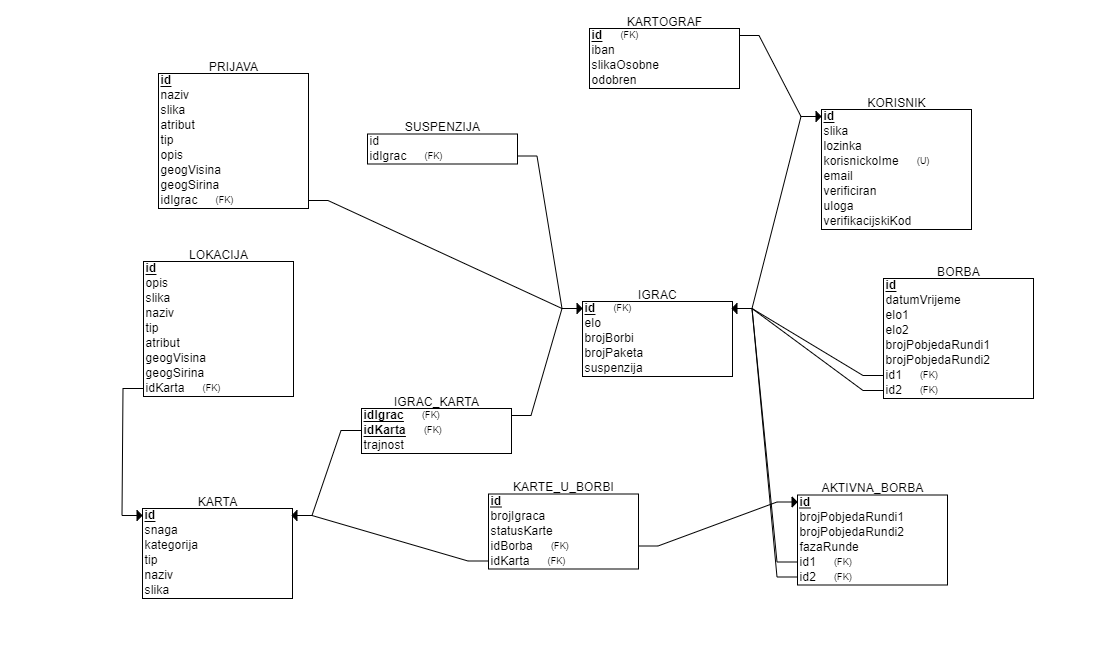
\includegraphics[width=\textwidth]{slike/relacijskiDijagram.png}
			\centering
			\caption{Dijagram baze podataka}
			\label{fig:promjene}
		\end{figure}

		\eject


		\section{Dijagram razreda}

		Na slikama 4.2, 4.3, 4.4 i 4.5 su prikazani razredi koji pripadaju \textit{backend} dijelu \textit{Controller-Service-Repository} arhitekture. Razredi prikazani na slici 4.1 pripadaju \textit{Controlleru}, te su metode u tim razredima zadužene za funkcionalnost. Metode implementirane u tim razredima manipuliraju s DTO \textit{(Data transfer object)}, a oni su dohvaćeni pomoću metoda implementiranih u Model razredima. Metode implementirane u Controller razredima vraćaju JSON datoteke s javascript status kodom.

		\begin{figure}[H]
			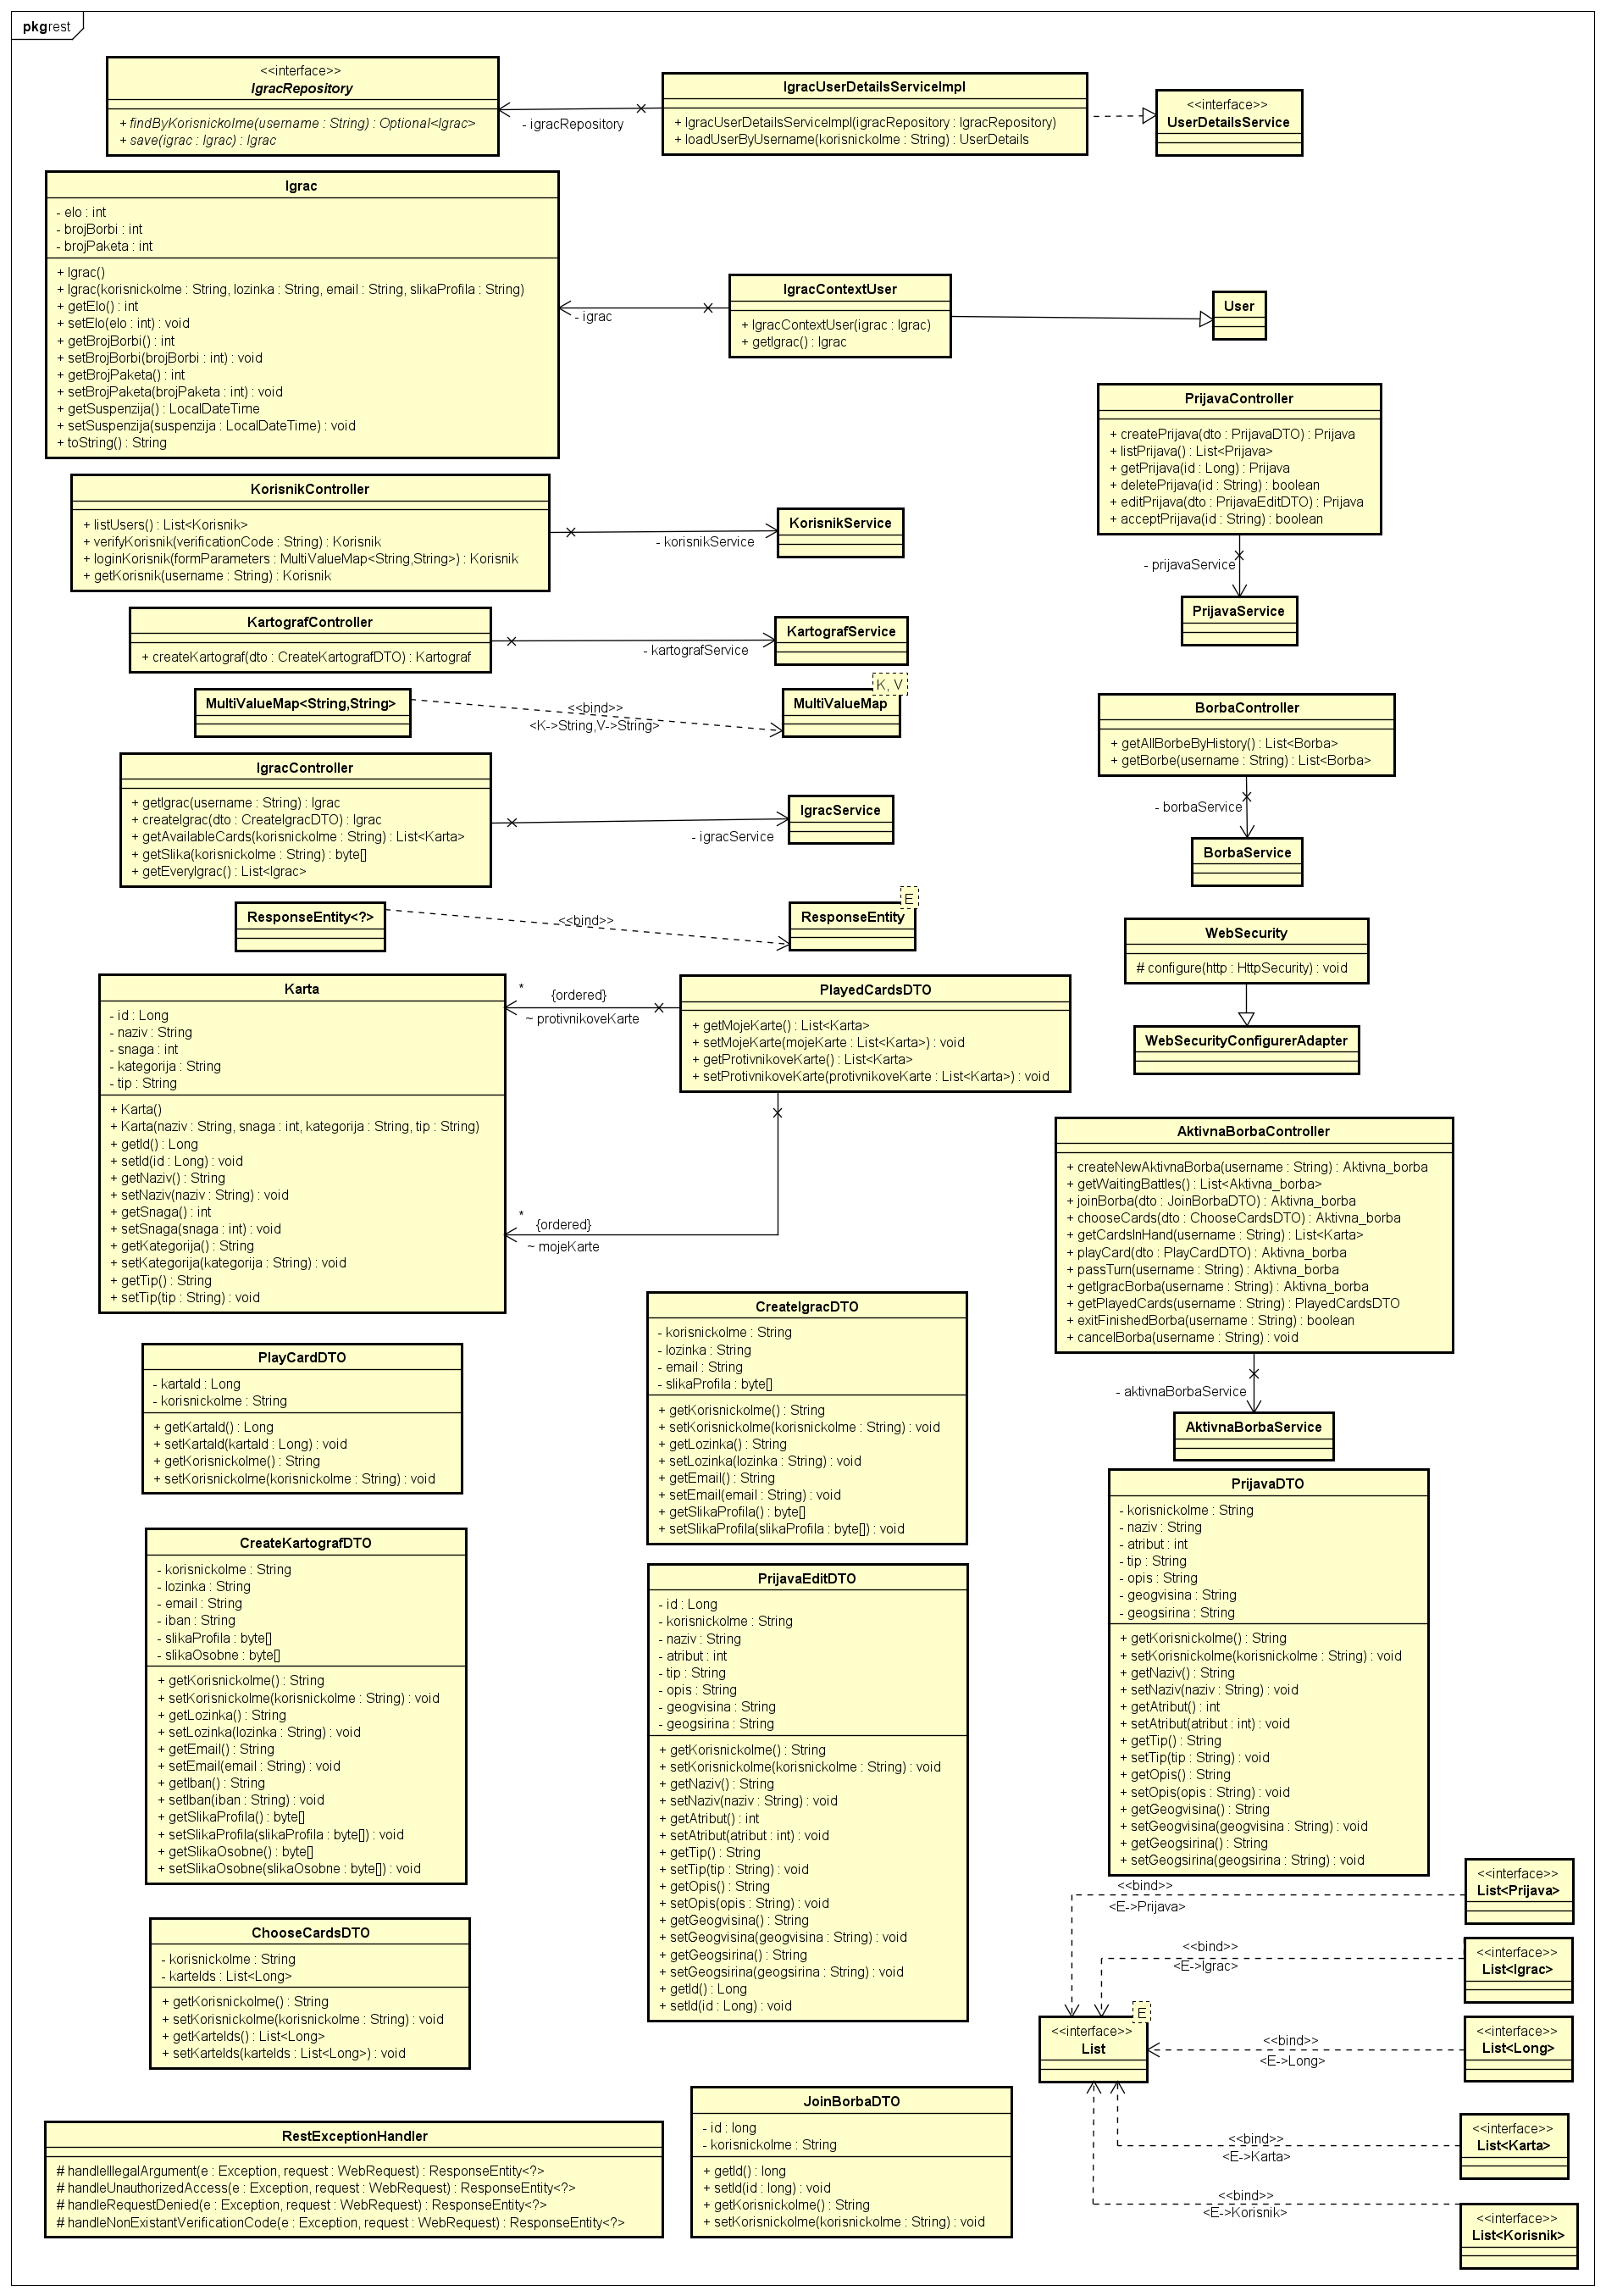
\includegraphics[width=\textwidth]{slike/Rest.png}
			\centering
			\caption{Dijagram razreda – Rest}
			\label{fig:promjene}
		\end{figure}

		\begin{figure}[H]
			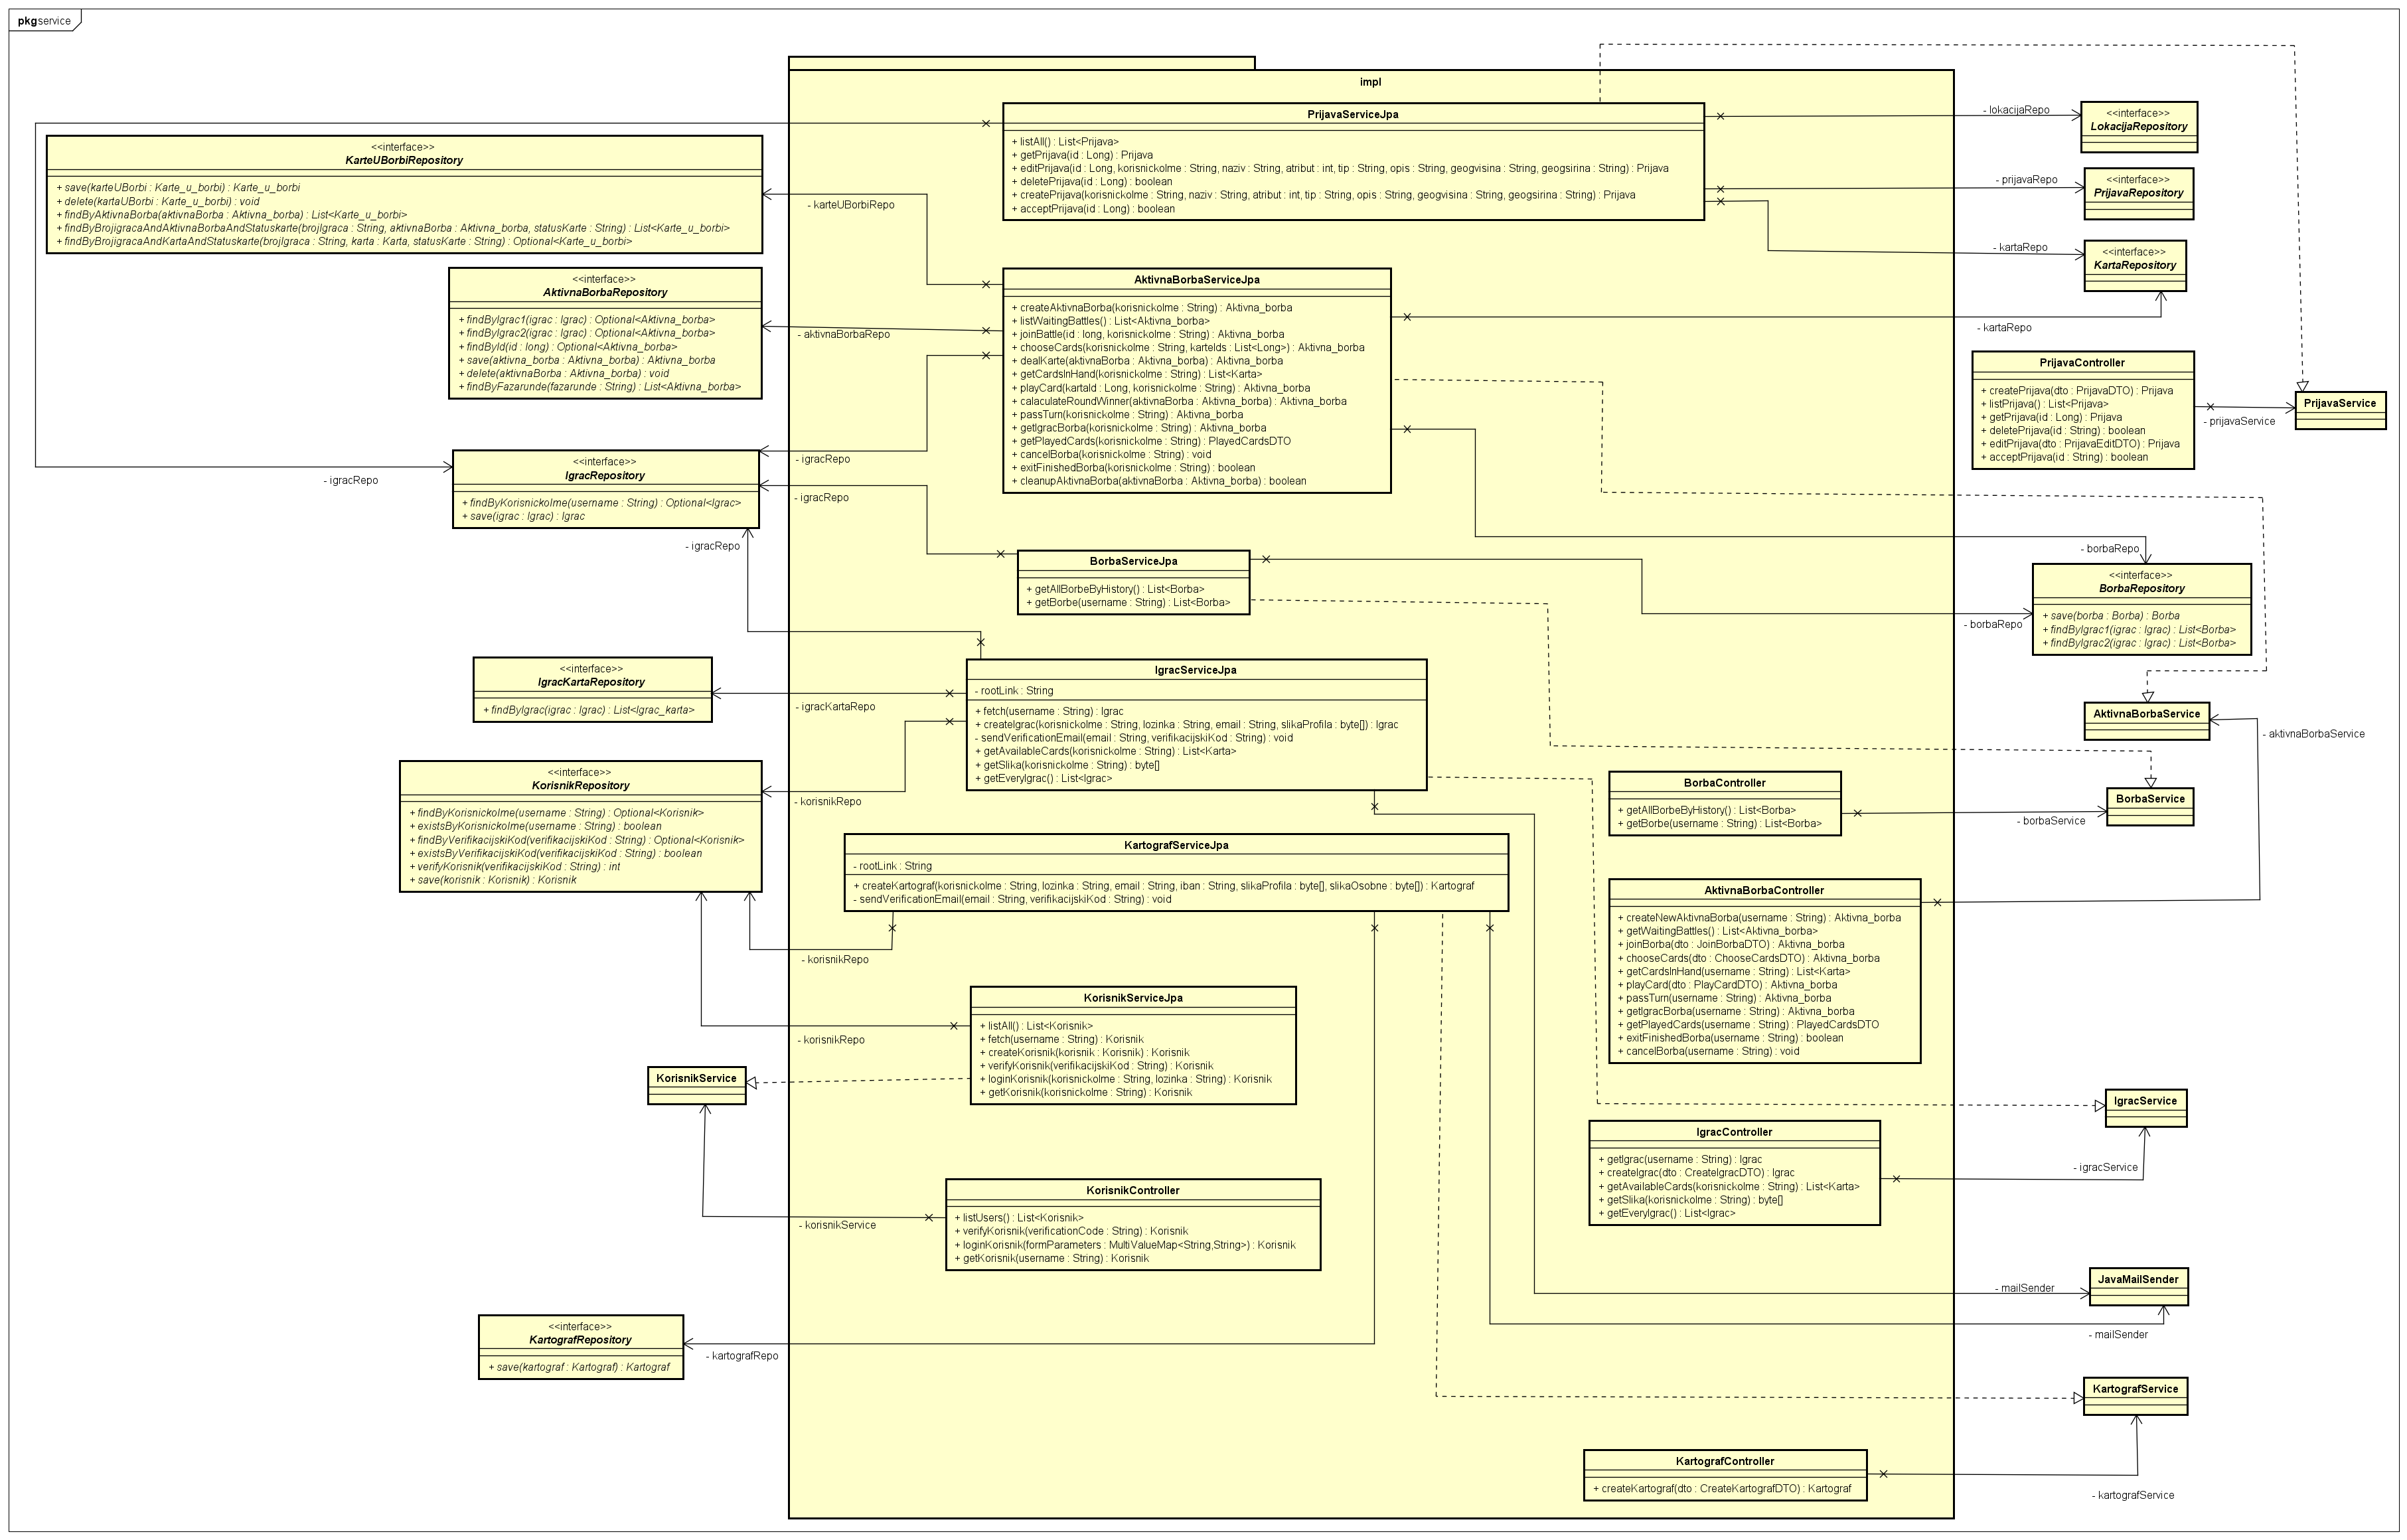
\includegraphics[width=\textwidth]{slike/service.png}
			\centering
			\caption{Dijagram razreda – Service}
			\label{fig:promjene}
		\end{figure}

		\begin{figure}[H]
			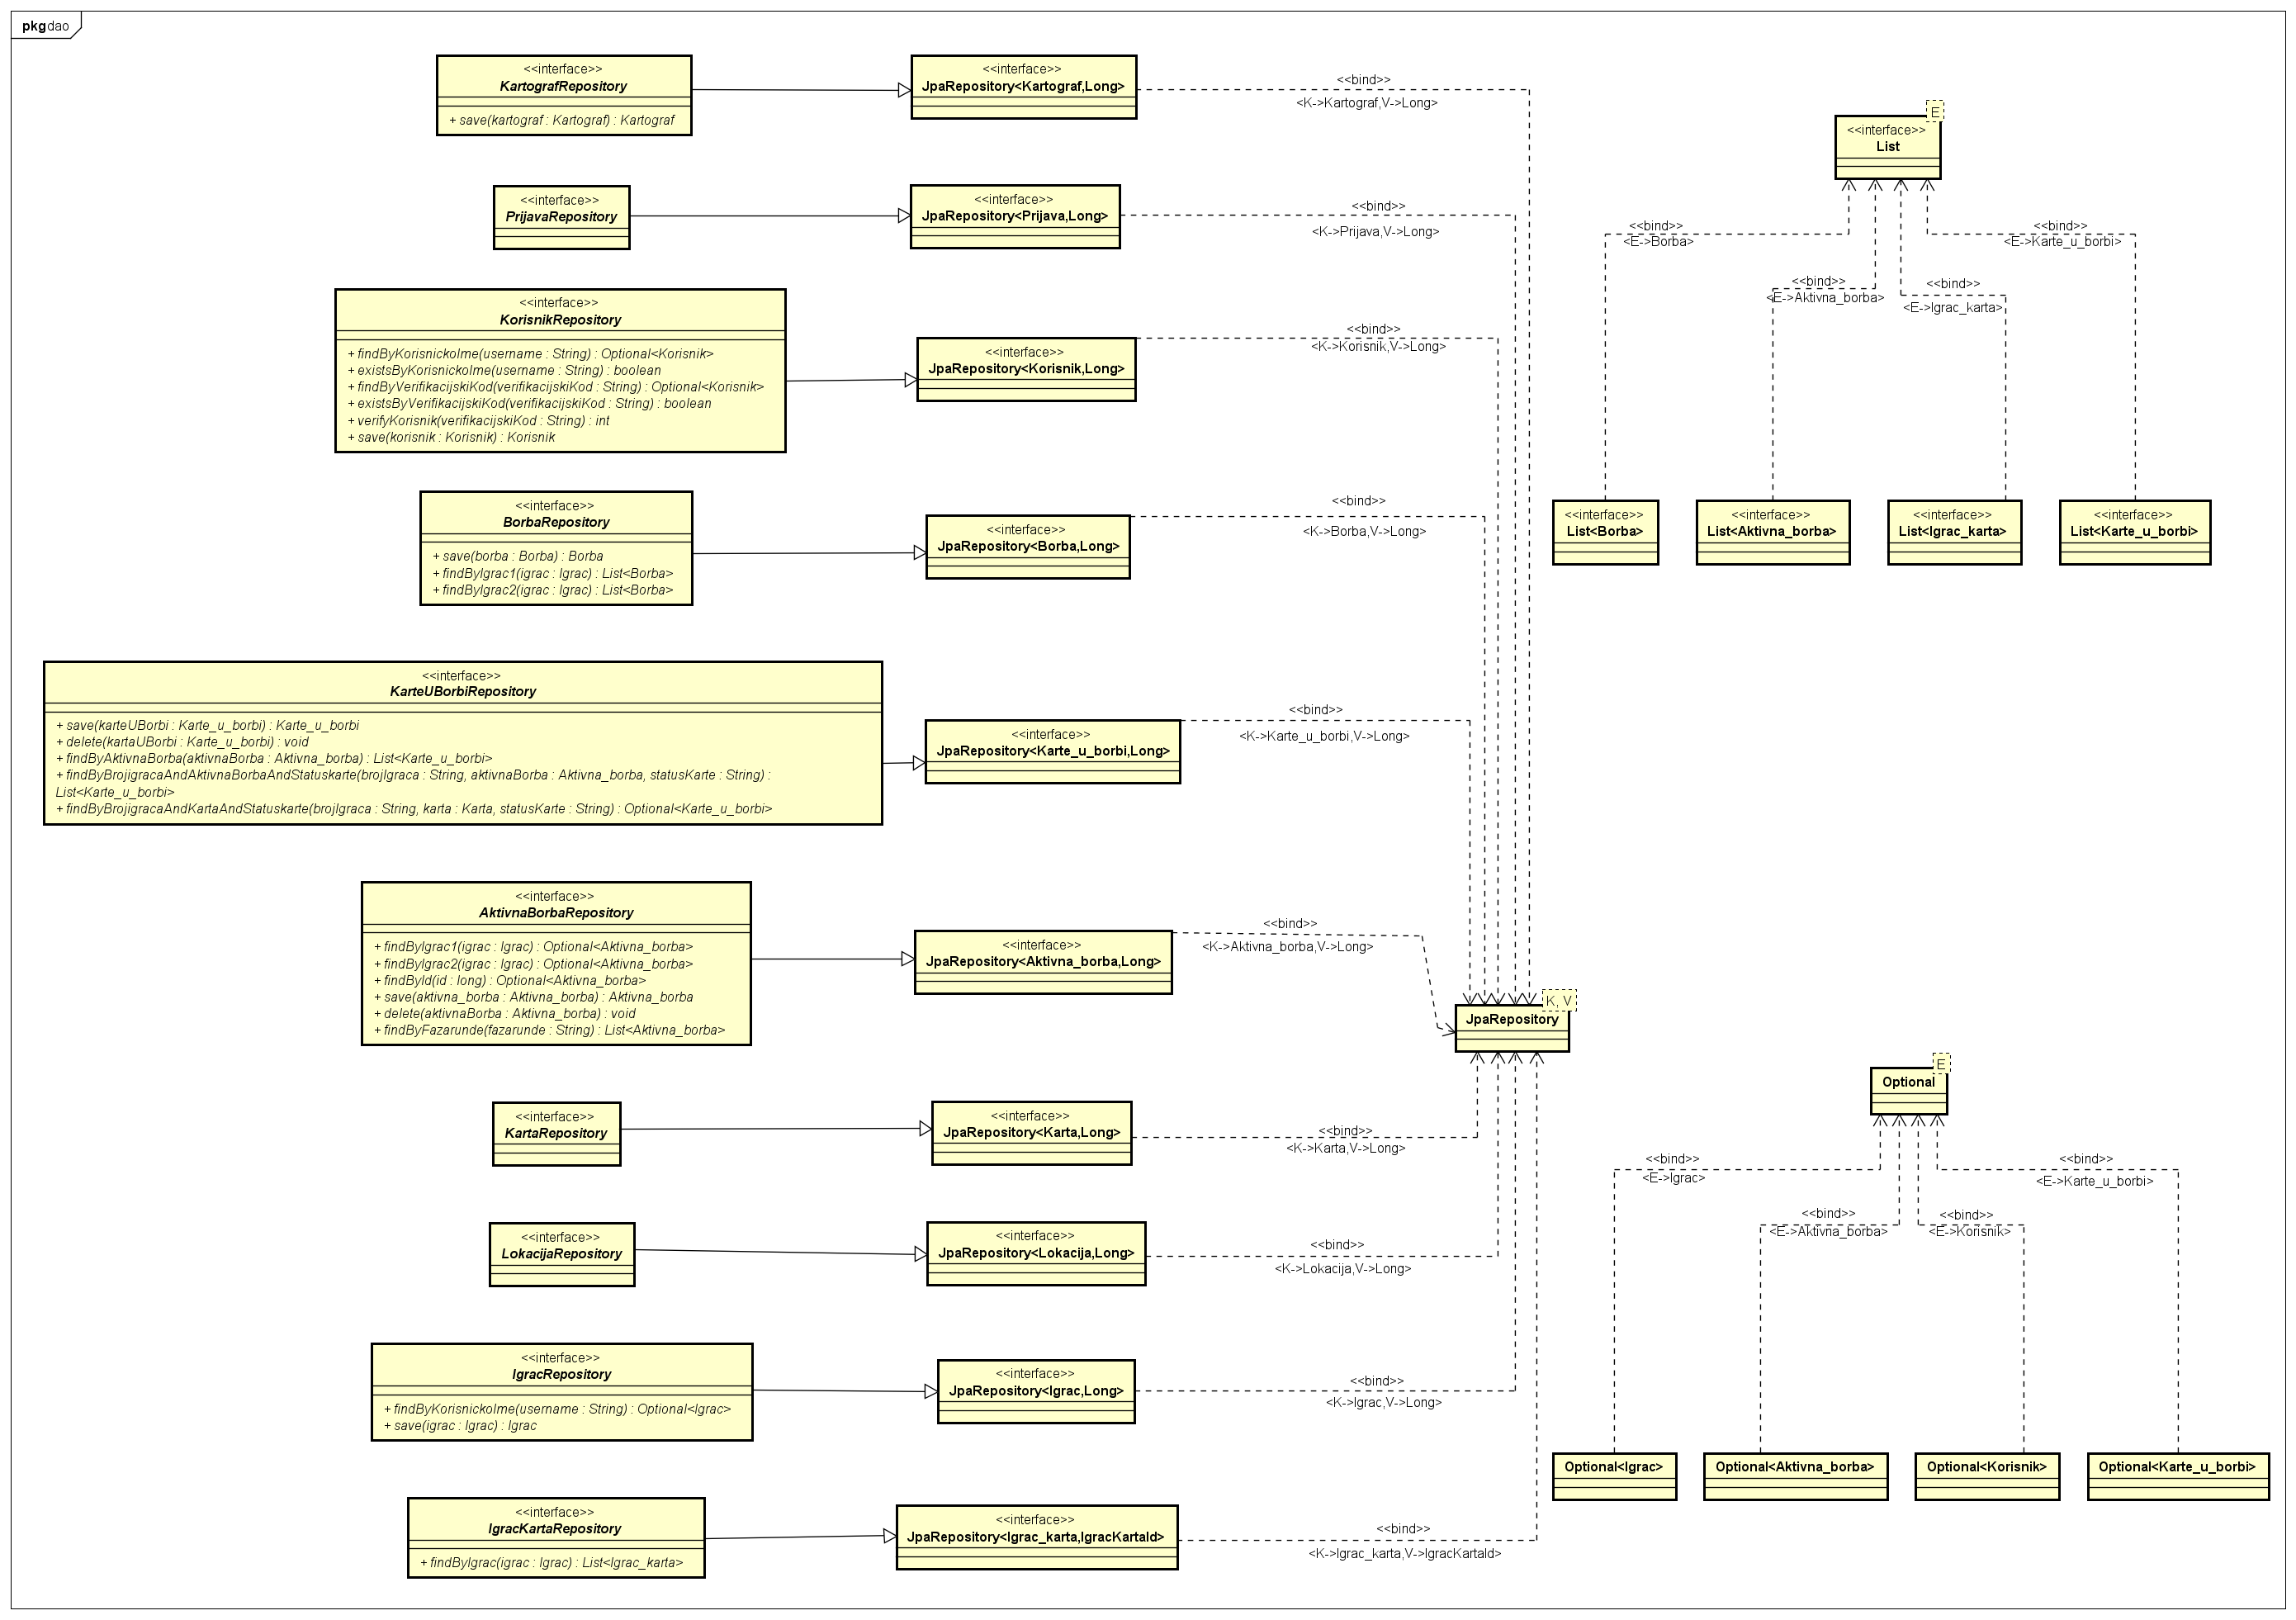
\includegraphics[width=\textwidth]{slike/Dao.png}
			\centering
			\caption{Dijagram razreda – Dao}
			\label{fig:promjene}
		\end{figure}
		\pagebreak
		Model razredi preslikavaju strukturu baze podataka u aplikaciji. Implementirane metode direktno komuniciraju s bazom podataka te vraćaju tražene podatke. Razred Korisnik predstavlja neregistriranog korisnika koji se može registrirati u sustav unoseći osnovne informacije. Razred Igrač predstavlja registriranog korisnika koju može koristiti osnovne funkcionalnosti sustava poput ulaska u borbu i pregleda svojih karata. Razred Kartograf predstavlja kartografa koji je registriran u sustav. Razred Lokacija predstavlja lokaciju registriranu u sustavu koja se može odigrati u borbi kao karta, ako ju igrač ima u svojoj kolekciji. Borba predstavlja skup svih podataka i metoda koji se koriste u borbi između dva igrača.

		\begin{figure}[H]
			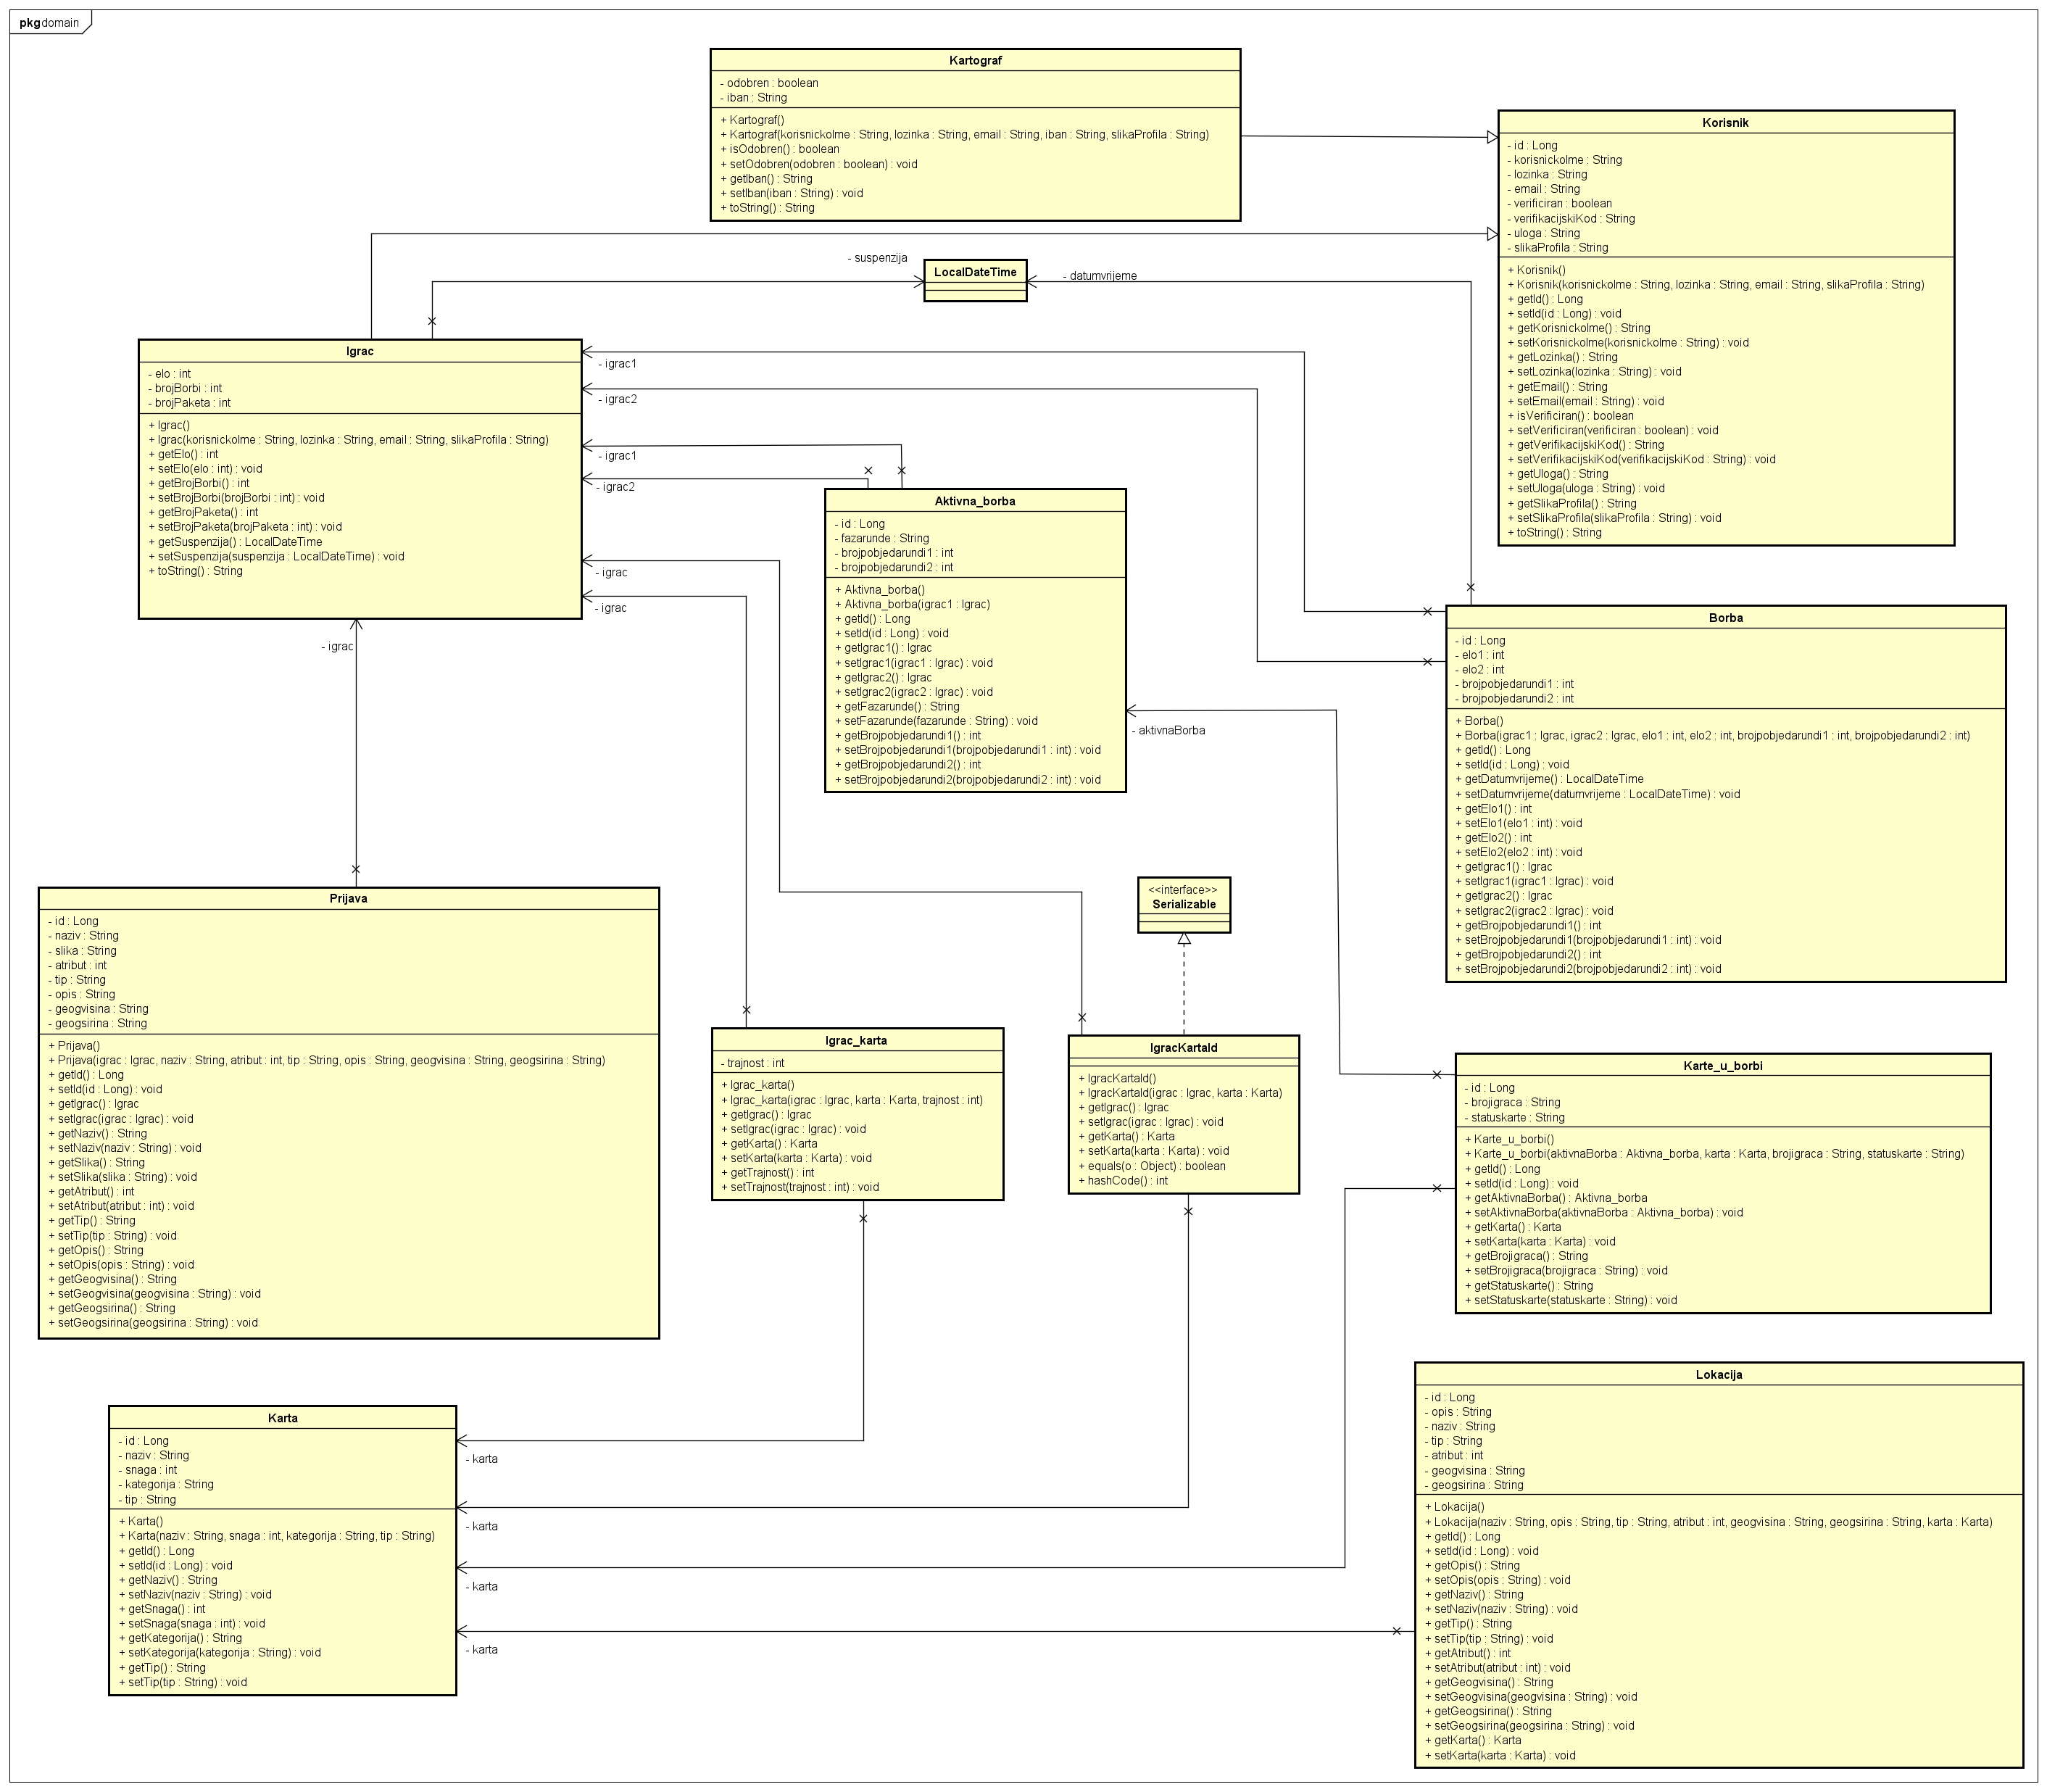
\includegraphics[width=\textwidth]{slike/Domain.png}
			\centering
			\caption{Dijagram razreda – Domain}
			\label{fig:promjene}
		\end{figure}


		\eject

		\section{Dijagram stanja}
		Dijagram stanja prikazuje stanja objekta te prijelaze iz jednog stanja u drugo temeljene na događajima. Na slici 4.6 prikazan je dijagram stanja za registriranog korisnika. Nakon prijave, klijentu se prikazuje glavni izbornik preko kojeg može ući u borbu, pogledati svoje karte i pogledati profil drugog igrača. Osim toga, preko alatne trake može pogledati poredak igrača, globalnu statistiku, početnu stranicu, urediti svoj profil i prijaviti novu lokaciju. Prije ulaska u borbu korisnik odabire između stvaranja vlastite borbe, gdje čeka protivnika da mu se pridruži, i pridruživanja borbi koju je protivnik pokrenuo. Pregledom tuđeg profila, korisnik može vidjeti protivnikove prošle borbe i karte koje ima u svojoj kolekciji. Kod prijave nove lokacije korisnik odabire lokaciju, daje joj ime, snagu, tip i opis.
		\begin{figure}[H]
			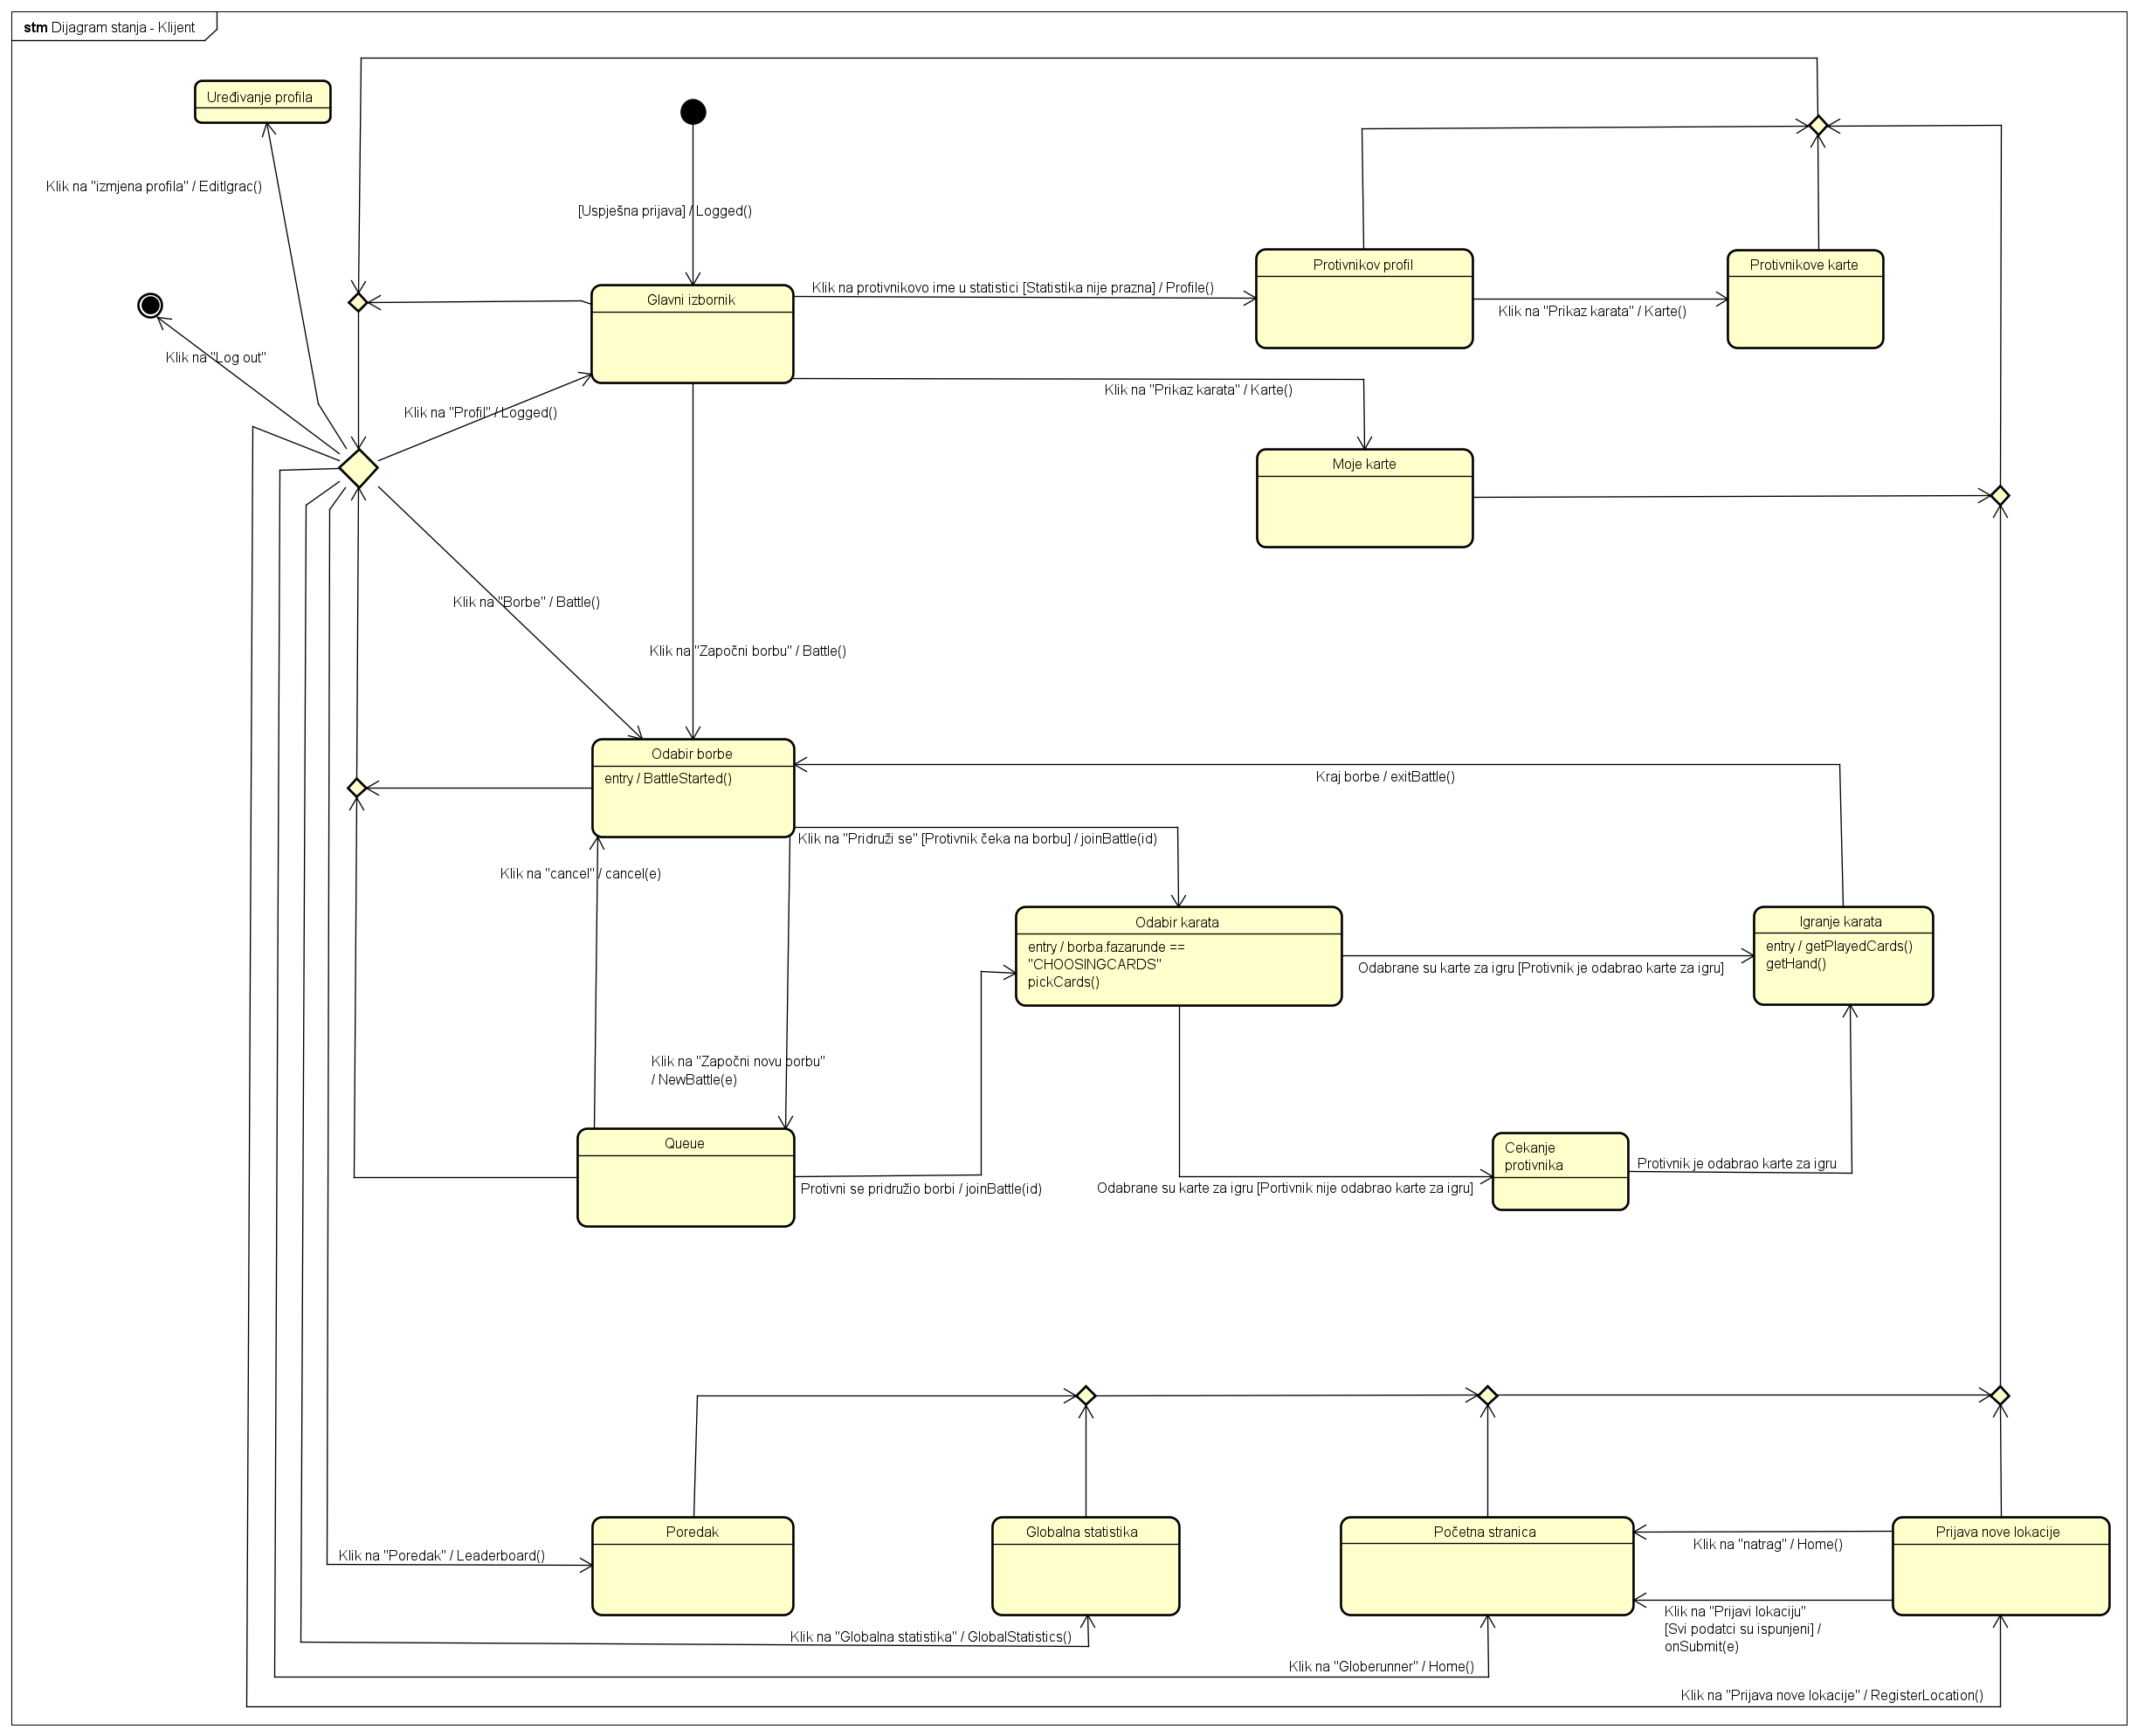
\includegraphics[width=\textwidth]{slike/Dijagram_stanja_-_Klijent.png}
			\centering
			\caption{Dijagram stanja}
			\label{fig:promjene}
		\end{figure}

		\eject

		\section{Dijagram aktivnosti}

		Dijagram aktivnosti primjenjuje se za opis modela toka upravljanja ili toka podataka. Na slici 4.7 je prikazana dijagram aktivnosti za borbu. Borba započinje biranjem 15 karata iz korisnikove kolekcije. Nakon što su oba igrača odabrala karte započinje borba, dodijeljeno im je 5 nasumičnih karata te po jedna karta nakon svake odigrane runde. Svaku rundu se mijenja koji igrač igra prvi, a prvu rundu aplikacija nasumično bira tko otvara igru. Prvi igrač igra životinju pa drugi nakon njega. Nakon toga se igra lokacija, koju igrači mogu, no ne moraju odigrati. Igrač koji prvi pobijedi dvije runde je pobjednik borbe. Na slici 4.8 je prikazana dijagram aktivnosti za kartografa. Nakon prijave u sustav, kartografu se prikažu sve prijavljene lokacije koje čekaju na njegovo odobrenje. Svaku prikazanu lokaciju kartograf može prihvatiti, obrisati, urediti ili odrediti najkraći put do lokacije.
		\begin{figure}[H]
			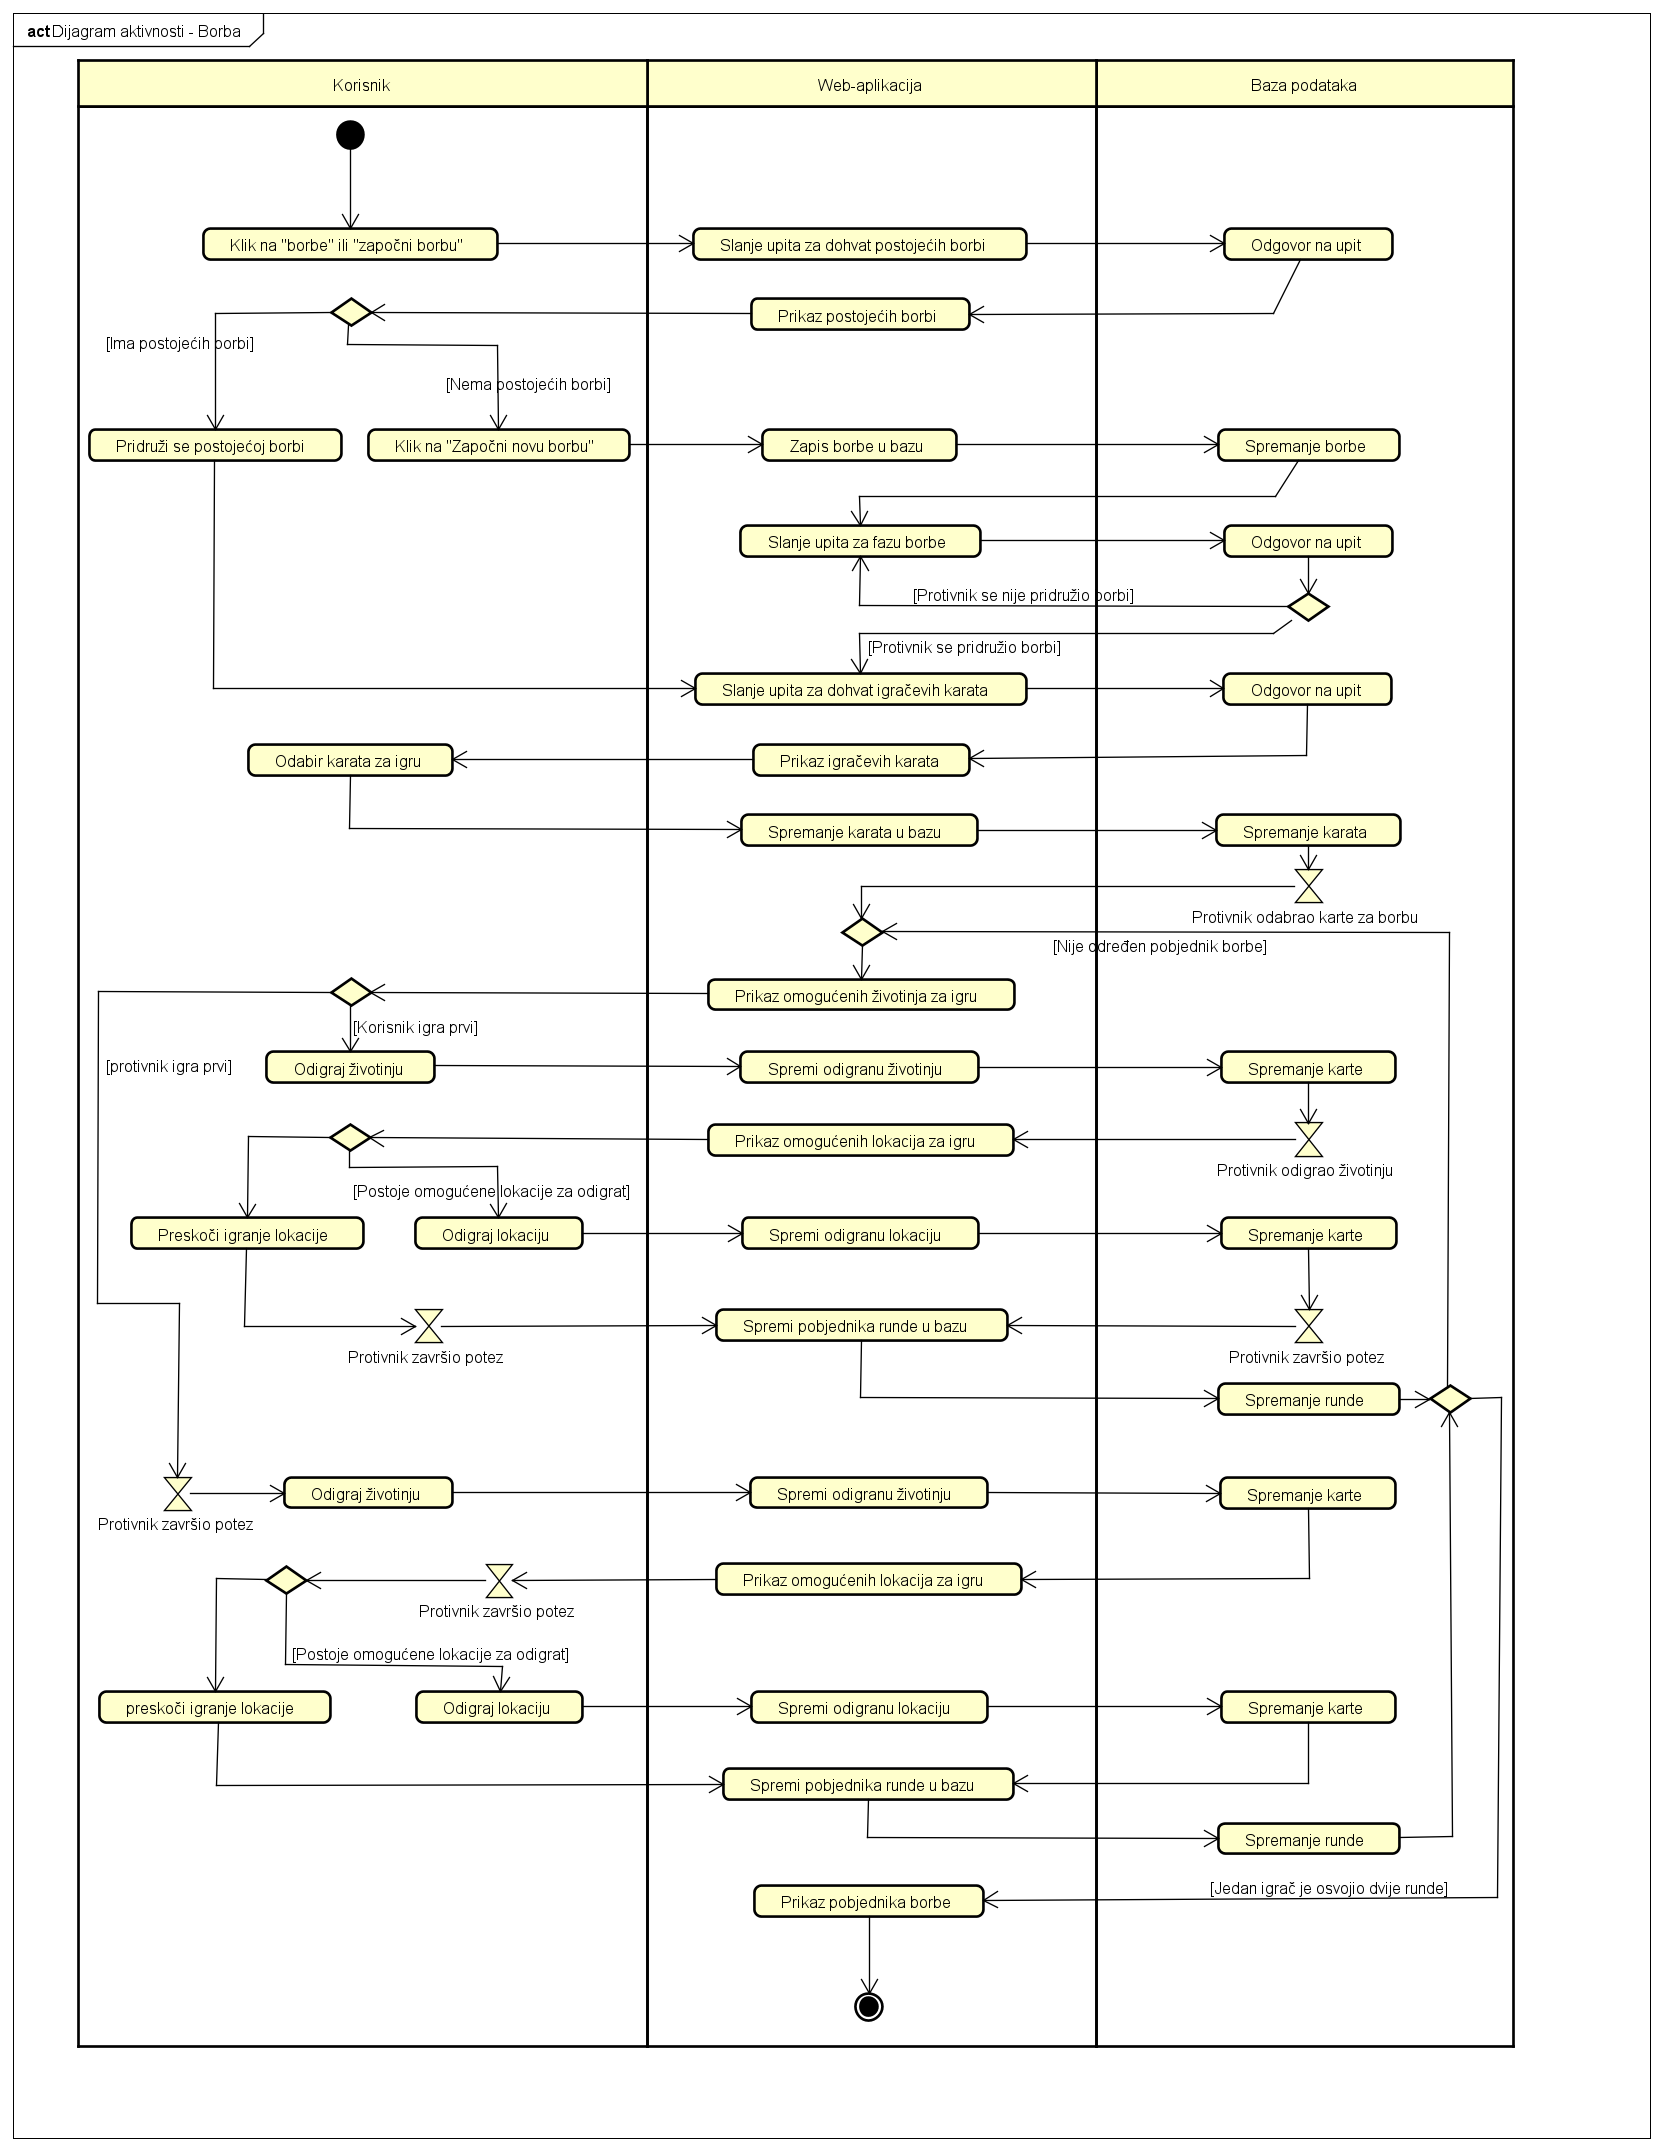
\includegraphics[width=\textwidth]{slike/Dijagram_aktivnosti_-_Borba.png}
			\centering
			\caption{Dijagram aktivnosti - Borba}
			\label{fig:promjene}
		\end{figure}
		\begin{figure}[H]
		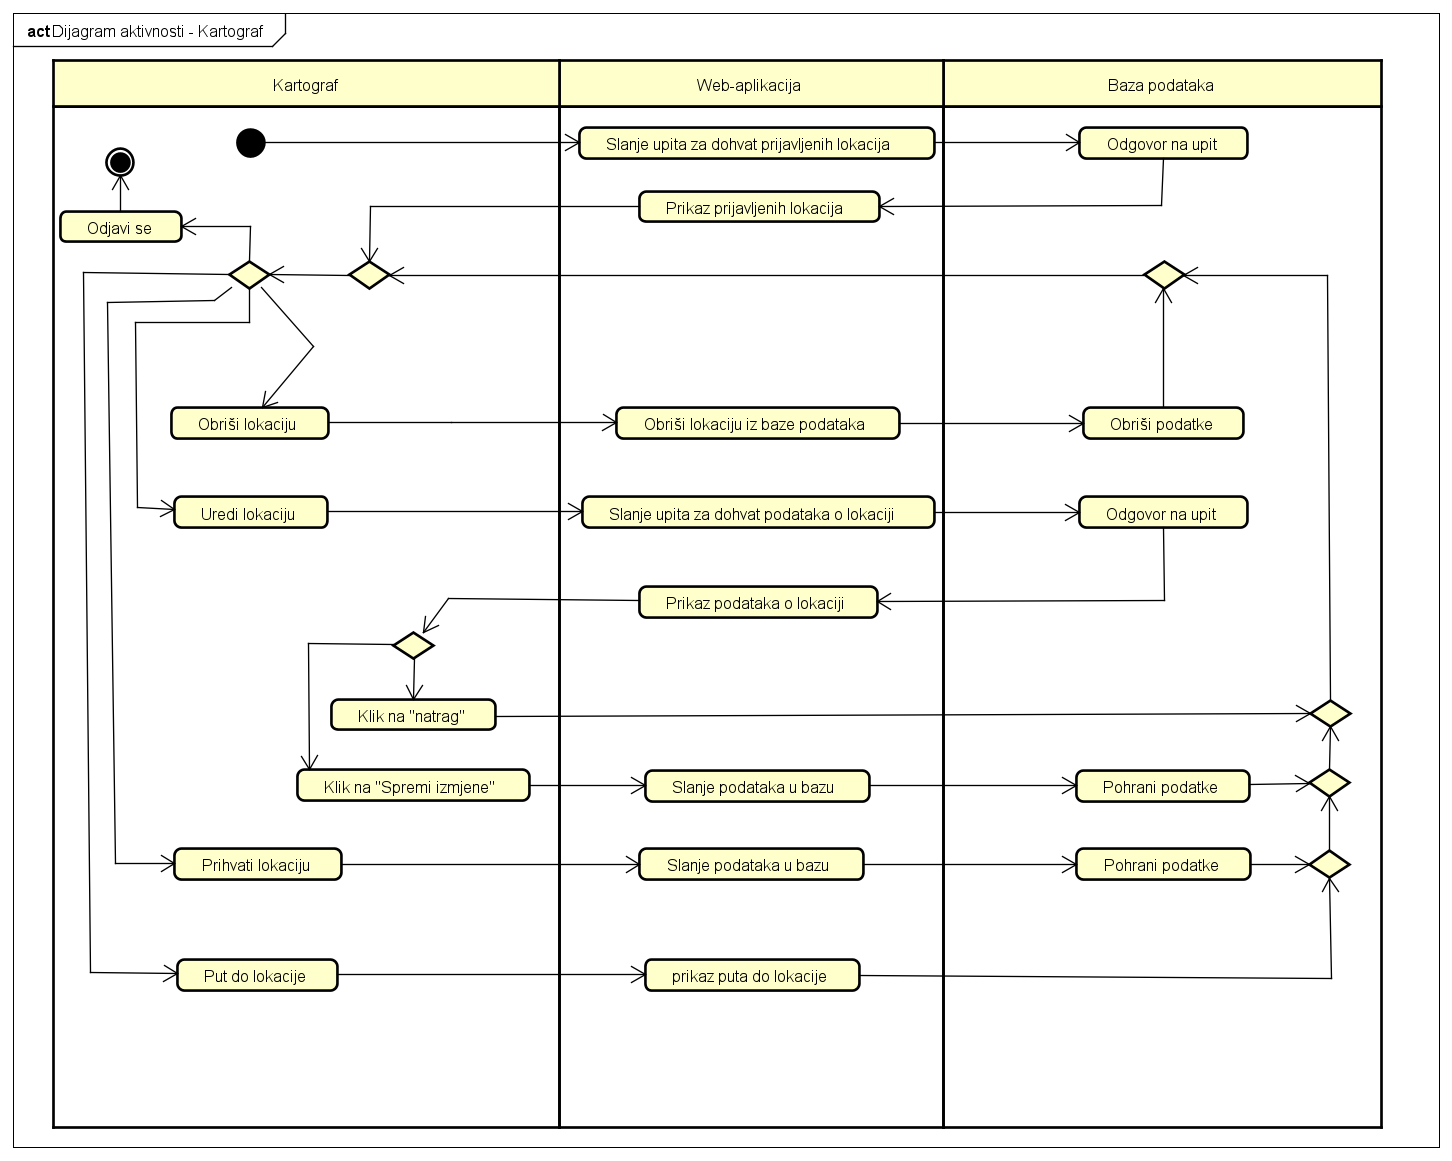
\includegraphics[width=\textwidth]{slike/Dijagram_aktivnosti_-_Kartograf.png}
		\centering
		\caption{Dijagram aktivnosti - Kartograf}
		\label{fig:promjene}
		\end{figure}

		\eject
		\section{Dijagram komponenti}
		Dijagram komponenti prikazan na slici 4.9 opisuje organizaciju i međuovisnost komponenti, interne strukture i odnose prema okolini. Sustavu se pristupa preko dva različita sučelja. Preko sučelja za dohvat CSS i JS datoteka poslužuju se datoteke koje pripadaju frontend dijelu aplikacije. App.js(Router) je komponenta koja na upit s url određuje koja datoteka će se poslužiti na sučelje. Frontend dio se sastoji od niza JavaScript datoteka koje su raspoređene u logičke cjeline nazvane po dijelu aplikacije za koji se koriste. Sve JavaScript datoteke ovise o React, Leaflet i Leaflet-routing-machine bibliotekama iz koje dohvaćaju gotove komponente. Preko sučelja za dohvat JSON podataka pristupa se REST API komponenti. REST API poslužuje podatke koji pripadaju backend dijelu aplikacije. JpaRepository je zadužen za dohvaćanje tablica iz baze podataka pomoću SQL upita. React-view komponenta preko dostupnih sučelja komunicira s Globerunner aplikacijom te ovisno o korisnikovim akcijama osvježava prikaz i dohvaća nove podatke i datoteke.
		\begin{figure}[H]
			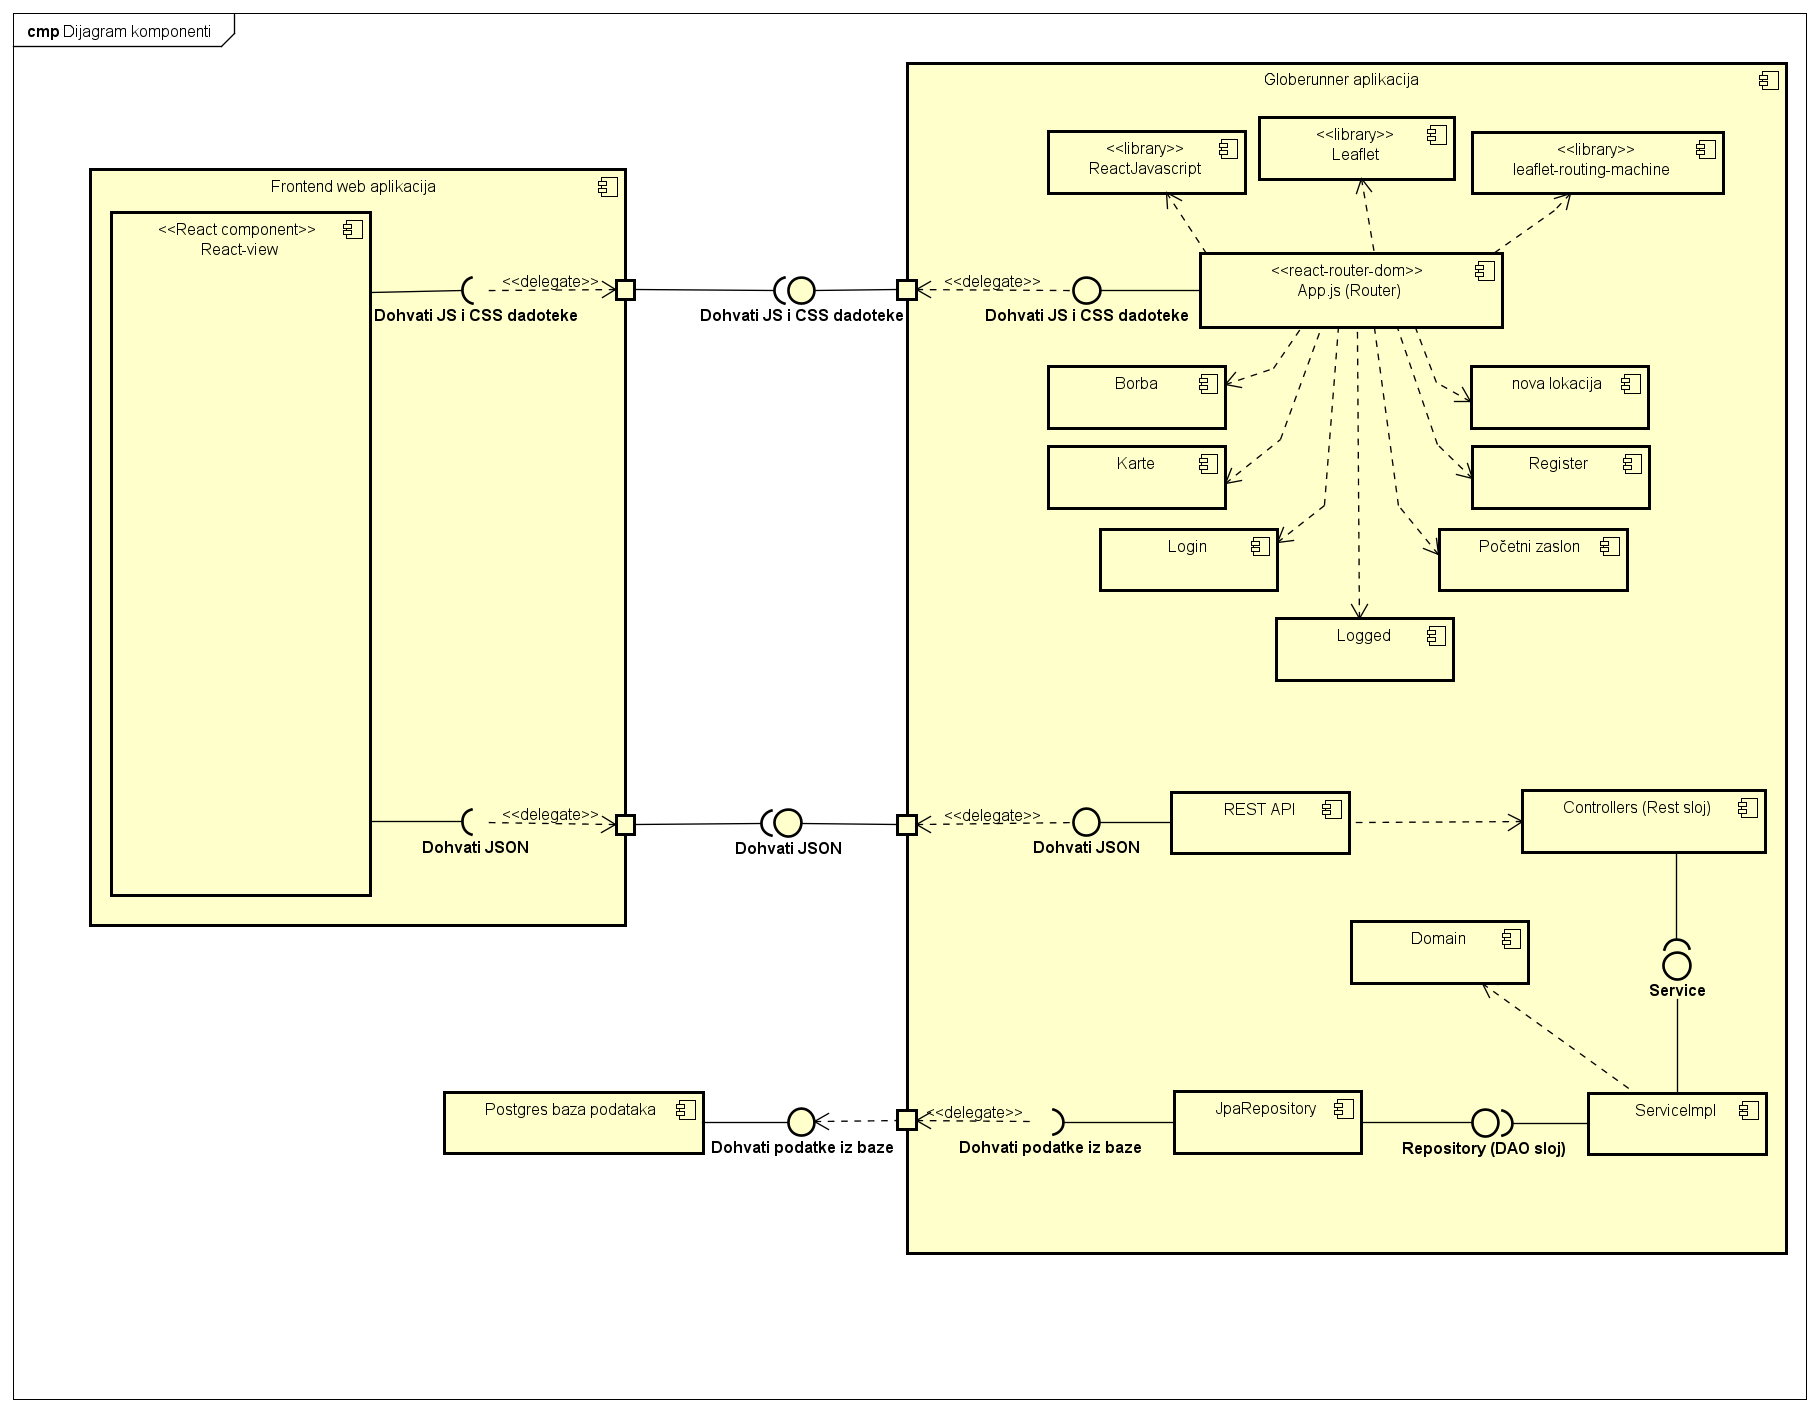
\includegraphics[width=\textwidth]{slike/Dijagram_komponenti.png}
			\centering
			\caption{Dijagram komponenti}
			\label{fig:promjene}
		\end{figure}
